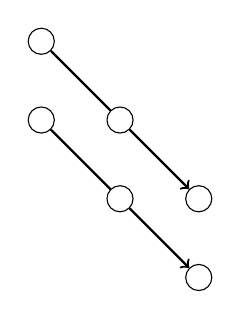
\begin{tikzpicture}[
    node/.style={circle, draw=black, fill=white, minimum size=6pt},
    arrow/.style={->, thick}
]

\node[node] (A1) at (0,1) {};
\node[node] (A2) at (1,0) {};
\node[node] (A3) at (2,-1) {};

\node[node] (B1) at (0,0) {};
\node[node] (B2) at (1,-1) {};
\node[node] (B3) at (2,-2) {};

\draw[arrow] (A1) -- (A2) -- (A3);
\draw[arrow] (B1) -- (B2) -- (B3);

\end{tikzpicture}